\documentclass[11pt]{scrartcl}

    \usepackage{ucs}
    \usepackage[utf8]{inputenc}
    \usepackage[T1]{fontenc}
    \usepackage[ngerman]{babel}
    \usepackage{amsmath,amssymb,amstext}
    \usepackage{graphicx}
    \usepackage{parskip}
    \usepackage{hyperref}
    \usepackage{float}
    \usepackage{subfiles}
    \usepackage{titling}
    \usepackage{ccicons}
    \usepackage{fontawesome}
    \usepackage{subfig}
    \usepackage[top=1in, bottom=1.25in, left=1.25in, right=1.25in]{geometry}
    \usepackage{xcolor}
    \usepackage{listings}
    \usepackage{natbib}
    \usepackage{enumerate}
    \usepackage{longtable}

    \lstset{basicstyle=\small,
      showstringspaces=false,
      commentstyle=\color{black},
      keywordstyle=\color{blue}
    }

    \bibliographystyle{unsrtnat}
    \graphicspath{{images/}{images/Antrieb/}{images/Fahrdaten}{images/Maschinentechnik}{images/Objekterkennung}{images/Stromversorgung}{images/Vision}}


        %\title{Dokumentation - PREN}
        \title{Schlussdokumentation PREN1 Gruppe 28}
        \author{A. Rebsamen, J. Grepper, M. Omlin, \\ M. Schöni, P. Marty, S. Ineichen}
        \date{\today{}, Luzern}

    \begin{document}

        \begin{titlingpage}
            \begin{center}
                \begin{Huge} %Exakter Modulnamen und Modulnamen ausgeschrieben
                    TA.BA{\_}PREN1.H1801 \\
                    \textbf{\thetitle} \\
                \end{Huge}
                \vspace{0.5cm}
                \begin{huge} %Author-Variable
                    \theauthor \\
                \end{huge}
                \vspace{0.5cm}
                \vspace{1cm}
                \begin{figure}[H] %Titelbild
                    \centering
                    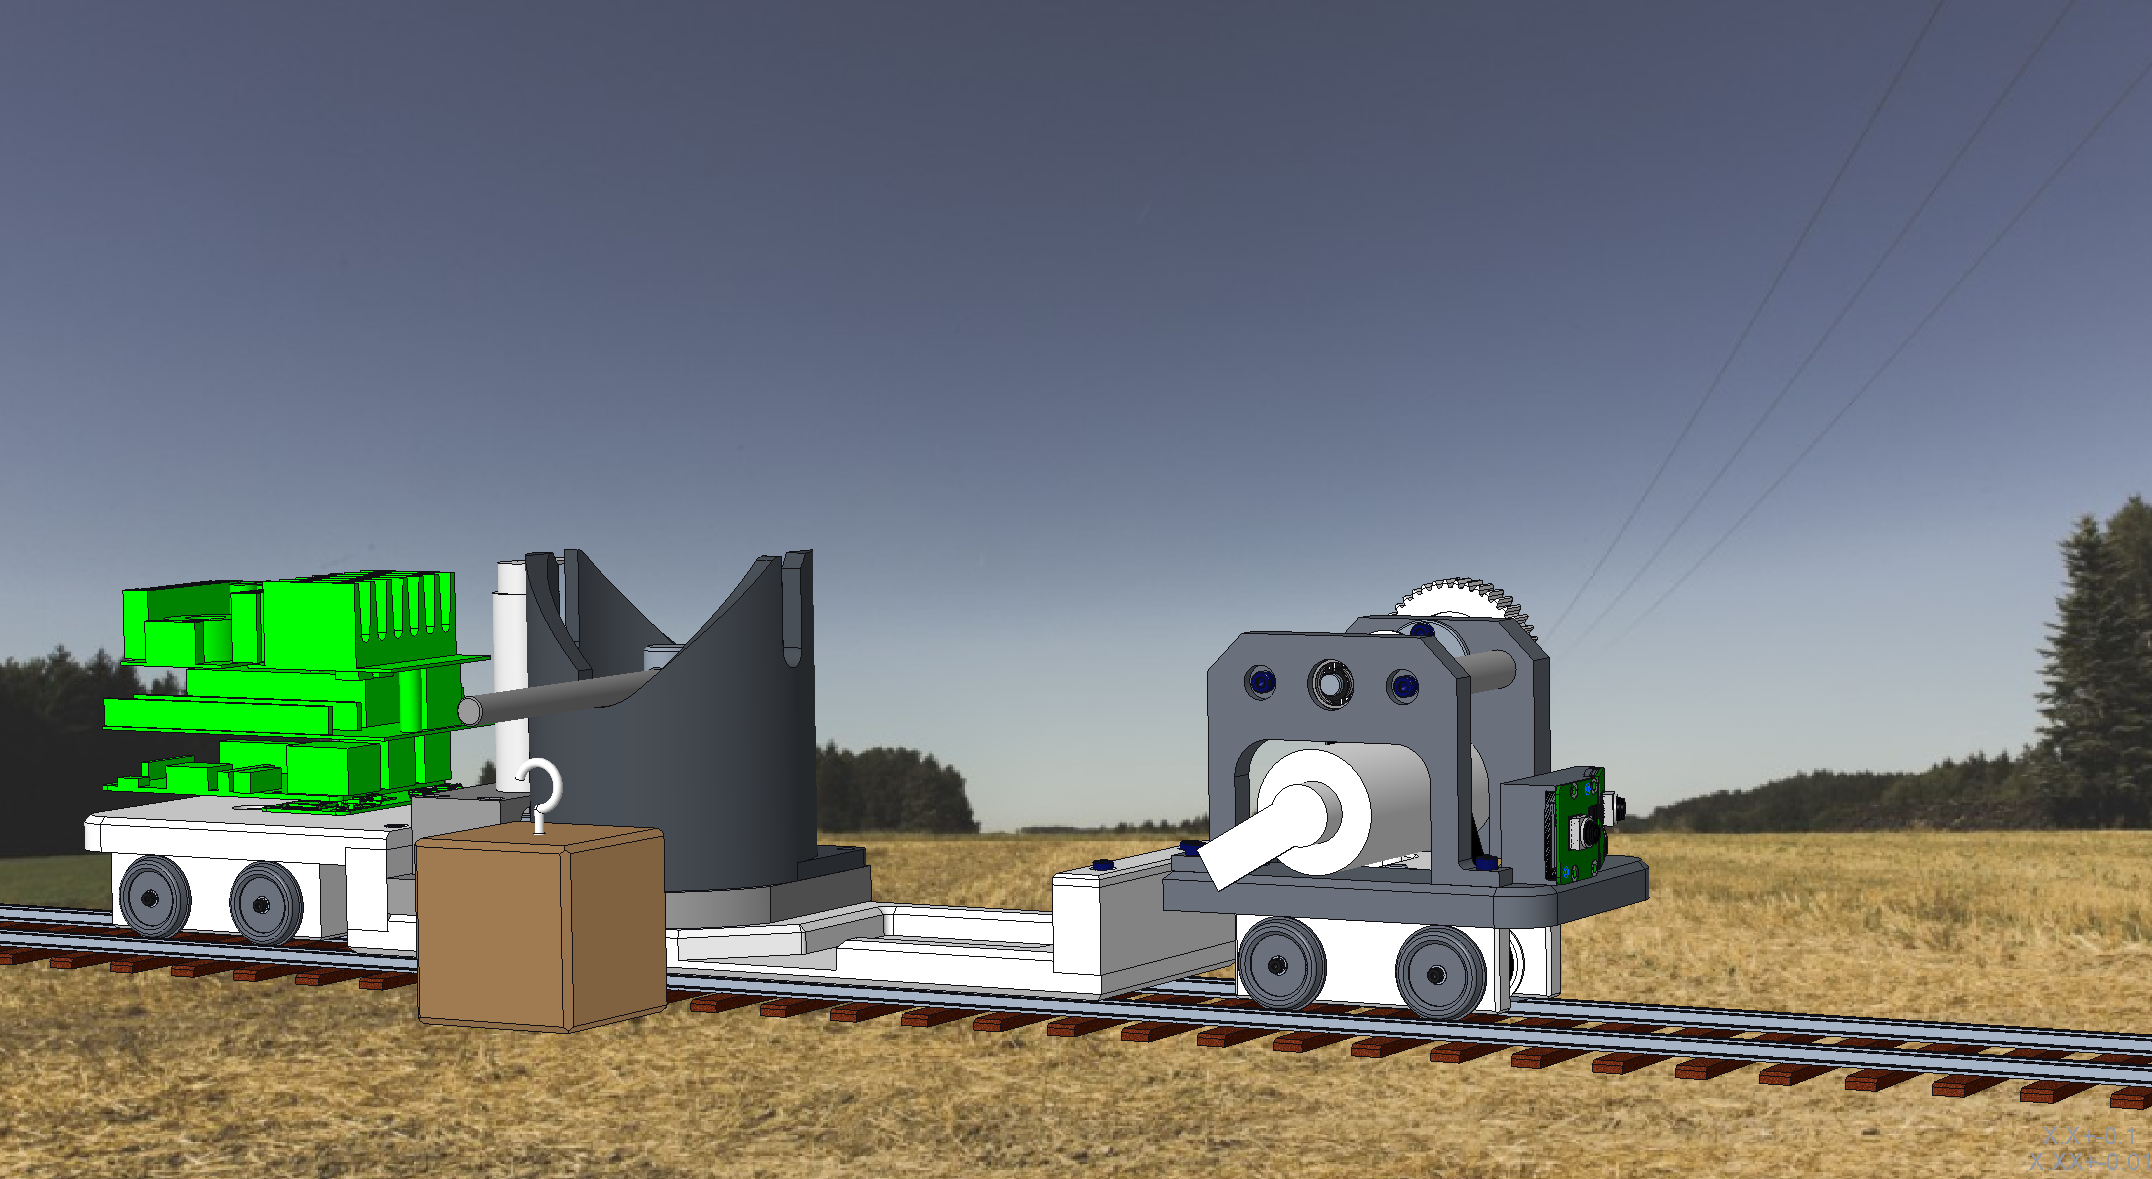
\includegraphics[width=0.8\textwidth]{images/uebersicht_Zug.png}
                \end{figure}
                \vspace{0.5cm}
                \begin{huge} %Datumsvariable
                    \thedate
                \end{huge}
            \end{center}
        \end{titlingpage}


        %Inhaltsverzeichnis
        \tableofcontents
        \clearpage

        \section{Management Summery}
        \subfile{sections/01_ManagementSummery/managementSummery.tex}
        \clearpage
        \section{Einleitung}
        \subfile{sections/02_Einleitung/einleitung.tex}
        \clearpage
        \section{Lösungskonzepte}
        \subfile{sections/03_Loesungskonzepte/loesungskonzepte.tex}
        \clearpage
        \subfile{sections/03_Loesungskonzepte/Ablauf.tex}
        \clearpage
        \subfile{sections/03_Loesungskonzepte/Fahrwerk.tex}
        \clearpage
        \subfile{sections/03_Loesungskonzepte/Wuerfeltransport.tex}
        \clearpage
        \subfile{sections/03_Loesungskonzepte/akustik.tex}
        \clearpage
        \subfile{sections/03_Loesungskonzepte/beschleunigung.tex}
        \clearpage
        \subfile{sections/03_Loesungskonzepte/Elektronik.tex}
        \clearpage
        \subfile{sections/03_Loesungskonzepte/signalerkennung.tex}
        \clearpage
        \subfile{sections/03_Loesungskonzepte/gleiserkennung.tex}
        \clearpage
        \subfile{sections/03_Loesungskonzepte/Interface.tex}
        \clearpage
        \subfile{sections/03_Loesungskonzepte/steuerungssoftware.tex}
        \clearpage
        \section{Projektmanagement}
        \subfile{sections/04_Projektmanagement/projektmanagement.tex}
        \clearpage
        \section{Schlussdiskussion}
        \subfile{sections/05_Schlussdiskussion/schlussdiskussion.tex}
        \clearpage
        %\section{Anhang}
        %\subfile{sections/06_Anhang/anhang.tex}
        %\clearpage
        \section{Verzeichnisse}
        \listoffigures
        \listoftables
        \bibliography{diverses/literatur-lib}

    \end{document}
